\documentclass[11pt,a4paper]{article}
\usepackage[utf8]{inputenc}
\usepackage[T1]{fontenc}
\usepackage{lmodern}
\usepackage[a4paper,margin=2cm]{geometry}
\usepackage{xcolor}
\usepackage{tikz}
\usetikzlibrary{arrows.meta}
\definecolor{kfrblue}{HTML}{1F5C99}

\begin{document}
\thispagestyle{empty}

% ============ Reflexion ============
\begin{center}
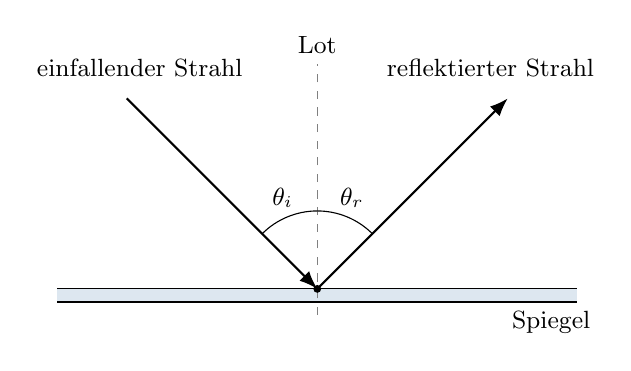
\begin{tikzpicture}[>=Latex, scale=1.1]
  % Spiegelfläche
  \draw[thick] (-3,0) -- (3,0);
  \fill[kfrblue!15] (-3,-0.15) rectangle (3,0);
  \draw[thick] (-3,-0.15) -- (3,-0.15);
  \node[below] at (2.7,-0.15) {\small Spiegel};

  % Lot (Normale)
  \draw[dashed, gray] (0,-0.3) -- (0,2.6);
  \node[above] at (0,2.6) {\small Lot};

  % einfallender Strahl
  \draw[->, thick] (-2.2,2.2) -- (0,0);
  \node at (-2.05,2.55) {\small einfallender Strahl};

  % reflektierter Strahl
  \draw[->, thick] (0,0) -- (2.2,2.2);
  \node at (2.0,2.55) {\small reflektierter Strahl};

  % Winkelbögen
  \draw (0,0) ++(90:0.9) arc (90:135:0.9);
  \node at (-0.4,1.05) {\small $\theta_i$};
  \draw (0,0) ++(90:0.9) arc (90:45:0.9);
  \node at (0.4,1.05) {\small $\theta_r$};

  \node[circle,fill=black,inner sep=1pt] at (0,0) {};
\end{tikzpicture}
\end{center}

\vspace{1cm}

% ============ Brechung ============
\begin{center}
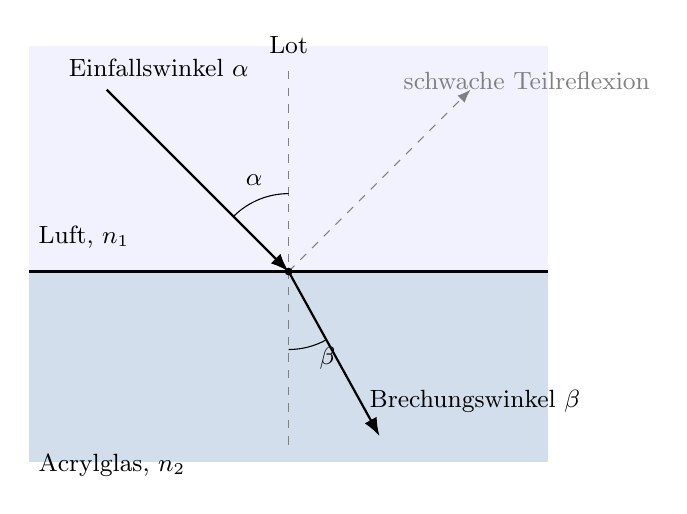
\begin{tikzpicture}[>=Latex, scale=1.1]
  % Medien
  \fill[blue!5] (-3,0) rectangle (3,2.6);
  \fill[kfrblue!20] (-3,-2.2) rectangle (3,0);
  \draw[thick] (-3,0) -- (3,0);
  \node[above right] at (-3,0.15) {\small Luft, $n_1$};
  \node[below right] at (-3,-2.0) {\small Acrylglas, $n_2$};

  % Lot (Normale)
  \draw[dashed, gray] (0,-2.0) -- (0,2.4);
  \node[above] at (0,2.4) {\small Lot};

  % einfallender Strahl
  \draw[->, thick] (-2.1,2.1) -- (0,0);
  \node at (-1.5,2.35) {\small Einfallswinkel $\alpha$};

  % gebrochener Strahl (zum Lot hin gebrochen, da n2>n1)
  \draw[->, thick] (0,0) -- (1.05,-1.9);
  \node at (2.15,-1.5) {\small Brechungswinkel $\beta$};

  % schwacher reflektierter Strahl (Teilreflexion)
  \draw[->, thin, gray, dashed] (0,0) -- (2.1,2.1);
  \node[gray] at (2.75,2.2) {\small schwache Teilreflexion};

  % Winkelbögen
  \draw (0,0) ++(90:0.9) arc (90:135:0.9);
  \node at (-0.4,1.05) {\small $\alpha$};
  \draw (0,0) ++(-90:0.9) arc (-90:-61:0.9);
  \node at (0.45,-1.0) {\small $\beta$};

  \node[circle,fill=black,inner sep=1pt] at (0,0) {};
\end{tikzpicture}
\end{center}

\end{document}
